\chapter{Employing GPUs in scientific algorithms}

The information age has brought a massive increase in the amount of data that is being collected and processed. The `data explosion' can be observed in virtually every field of computer science. In the scientific domain, this phenomenon is multiplied by increasingly powerful data-gathering devices (i.e., cytometers in bioinformatics, optic sensors in physics, seismometers in geology, etc.). The amount of data is simply too large to be processed in the required time. In order to alleviate this apparent pressure, the corresponding algorithm (which typically has super-linear time complexity) must be ported to massively parallel architectures, such as GPUs. The provided advantage can result in the ability to assess bigger data, use more detailed processing methods, or analyze the data in real time.

This chapter enumerates four selected scientific algorithms and discusses their challenges in porting to GPUs to enable higher performance.

\section{Hierarchical clustering with the Ma\-ha\-la\-no\-bis linkage}

In the field of bioinformatics, hierarchical clustering is a popular method for analyzing various types of data. 
In general, hierarchical clustering is an unsupervised machine learning method that aims to group the data points into clusters according to some linkage criterion.
It is an iterative method that starts with each data point being a cluster and, in each iteration, merges the two most similar clusters according to the linkage criterion until there is only one cluster.
There are many cluster linkage criteria to choose from, each with advantages and disadvantages. 
The most common linkage is the \emph{centroid linkage}, which computes the distance between the clusters centroids (the mean points).
In analyzing single-cell cytometry data, hierarchical clustering with the Mahalanobis linkage has been shown to be the most suitable method.

Mahalanobis linkage uses \emph{Mahalanobis distance} to measure the similarity between clusters:
\begin{defn}[Mahalanobis distance]
    Suppose a probability distribution $C$ on $\R^d$ with mean $\bar{C} \in \R^d$ and a convariance matrix $\cov(C)$. If the matrix $\cov(C)$ is regular, we define the \emph{Mahalanobis distance} between $u \in \R^d$ and $C$ as
    \begin{equation}
    d_\text{Maha}(u,C) = \sqrt{(u-\bar{C})^T\cov(C)^{-1}(u-\bar{C})}.
    \end{equation}\label{eq01:maha}
\end{defn}

If we generalize a centroid of a cluster to a probability distribution, Definition~\ref{eq01:maha} can be used to define the Mahalanobis distance between a point and a cluster. To extend the definition to a distance between two clusters, we use the following equation:
\begin{equation}
    \delta_\text{Maha}(P,Q) = \frac{d_\text{Maha}(\bar{P},Q) + d_\text{Maha}(\bar{Q},P)}{2}
\end{equation}\label{eq01:maha_linkage}

To illustrate the measure of the Mahalanobis distance, let us suppose we have two elliptic clusters. In the means of the proximity, the measure favors such clusters that their ellipses are alongside rather than in a prolongation of one another [TODO] (see Figure~\ref{fig:ellipses}). 
Only when the objects of a cluster form a spherical shape, this dissimilairity measure is proportional to the Euclidean distance with a corresponding linkage.
This allows for a very natural formation of clusters in biological data. However, the benefits come with the increase in complexity materialized in the computation of covariance matrix, matrix inverse, and vector-matrix-vector multiplication in each distance evaluation.

\begin{figure}[h]
    \centering
    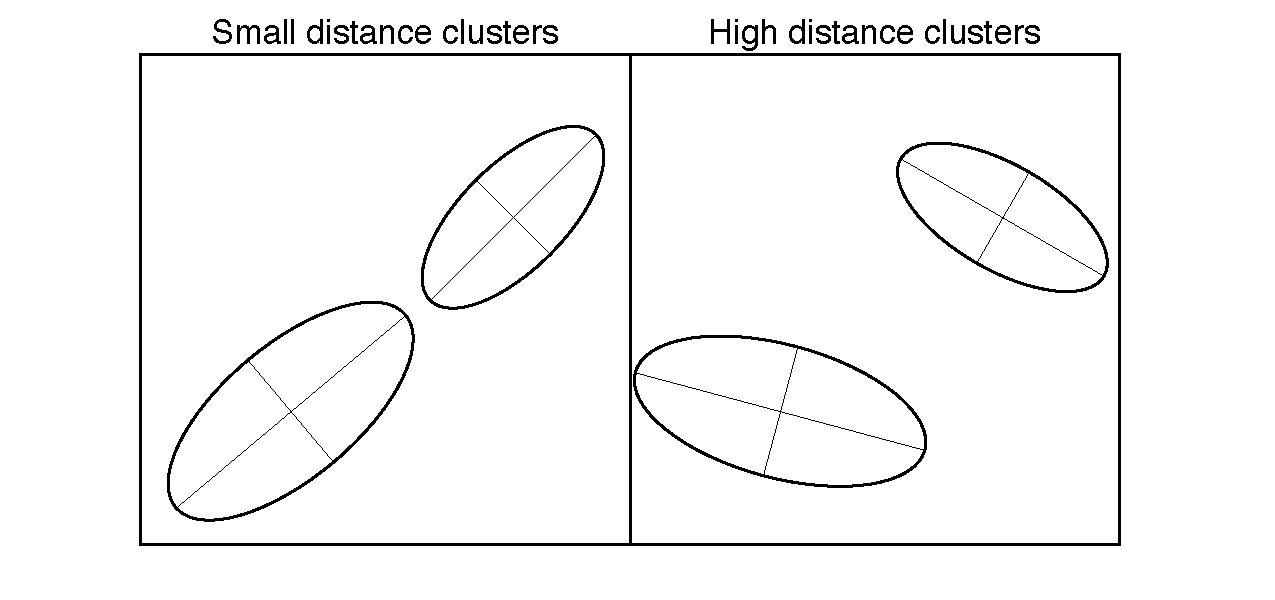
\includegraphics[width=0.6\textwidth]{img/ellipses.pdf}
    \caption{Two pairs of clusters with different similarities according to Mahalanobis distance}
    \label{fig:ellipses}
\end{figure}

\subsection{Algorithm complexity and the implementation}

Hierarchical Clustering (HC) is a well-known problem, and there are many algorithms that effectively solve it. Roughly, they can be divided into categories according to the data structures they employ [TODO]:
\begin{itemize}
    \item HC with a dissimilarity matrix --- the most straightforward approach; the dissimilarity matrix stores the distances between all pairs of clusters. This approach has a cubic time complexity and quadratic memory complexity.
    \item HC with a nearest neighbor array --- each cluster stores the index of its nearest neighbor. This approach trades a linear memory complexity for an asymptotic time complexity of $\mathcal{O}(d \cdot n^3)$.
    \item HC with an array of priority queues --- a more sophisticated solution, which reduces the time complexity to $\mathcal{O}(n^2 \log n)$.
\end{itemize}

C application \texttt{mhclust}, the original implementation of the Mahalanobis HC, uses the dissimilarity matrix. This approach is simple and allows for a straightforward implementation. However, the empirical data reveal the most significant limiting factor in the quadratic memory complexity. The Mahalanobis distance adds a multiplicative factor in $\mathcal{O}(d^2)$ to the memory complexity, so usually, the machine runs out of memory before the execution time reaches unreasonable limits.

As a solution to this limitation, we can assume \emph{in-place} variant of the HC with dissimilarity matrix, which discards the whole matrix and chooses the closest cluster pair by computing the distances ad-hoc. This increases the asymptotic time complexity to $\mathcal{O}(d \cdot n^3)$ assuming the Euclidean distance with centroid linkage.

Our work used the nearest neighbor array approach to achieve fewer distance computations per iteration on average while keeping the memory complexity linear. Notably, the algorithm complexity per iteration is quadratic only in the worst case, when each cluster's neighbor needs to be reevaluated. This case would correspond to constantly merging such cluster pairs that all the other clusters are neighboring. In practice, this is an atypical case, and the empirical data show that the number of neighbors to reevaluate is generally in the range of 10 to 100 for tested datasets with at most 1M of points.

Apart from the complex distance computation, the Mahalanobis HC suffers from the unbalanced nature of the algorithm. In the first iterations, the runtime is dominated by the distance computation in the data structure update. However, when the number of clusters decreases, the bottleneck becomes the covariance matrix computation of a merged cluster (with a time complexity of $\mathcal{O}(d^2 \cdot n)$). We used \emph{streams}, a CUDA abstraction for task parallelism on GPUs, to overlap the covariance matrix computation with the data structure update to keep GPU utilization high.

\subsection{Future work}

The Mahalanobis HC is a valuable method for analyzing cytometry data. However, since we published the optimized algorithm, there have been new additions to the GPU CUDA framework, which could be used to improve the performance of the algorithm further. Specifically, the whole Mahalanobis distance could be computed as a single \emph{Tensor} operation, drastically improving the application throughput. Another promising optimization would be to use \emph{CUDA Graph} to reduce the kernel launch overhead.


\section{Neighborhood-based dimensionality reduction}

Another approach to the analysis of multidimensional point-like cloud datasets is to reduce the dimensionality of the data to a lower (human-readable) dimension while preserving the local structure of the data. This approach is used in many areas of life sciences, such as microscopy imaging, population biology, and others. The most popular methods for dimensionality reduction are t-SNE and UMAP. Both these methods are nonlinear neighborhood embeddings and use a stochastic approach to find the optimal mapping. However, their applicability reaches a limit when increasing the scale or requiring real-time processing.

The EmbedSOM algorithm tries to tackle this limitation. It is based on self-organizing maps and uses a landmarks-based approach to reduce the computational complexity. Instead of computing all pairwise distances and stochastically optimizing the low-dimensional mapping, EmbedSOM uses a small set of landmarks to approximate the mapping. This allows for over a magnitude better performance while retaining the reasonable accuracy of the results. In our works, we followed up on the EmbedSOM algorithm and implemented it on GPUs to achieve real-time processing of large datasets, allowing for a semi-supervised dataset analysis.

\subsection{Backgound}

Algorithm~\ref{alg01:esom} highlights the overview of EmbedSOM algorithm. It assumes a set of $n$ high-dimensional (denoted with $d$) points $X \in \R^{n \times d}$, a set of $g << n$ high-dimensional landmarks $L \in \R^{g \times d}$, and a set of $g$ low-dimensional ($2$ for brevity) landmarks $l \in \R^{g \times 2}$. For each high-dimensional point, it finds a low-dimensional variant by selecting $k < g$ nearest landmarks, assigning them scores, and computing the optimal low-dimensional mapping according to the scores. The optimal mapping is computed by minimizing the sum of the differences between the distances of the high-dimensional point to the landmarks and the distances of the low-dimensional point to the landmarks. Because of the mapping nature, the minimization problem can be reduced to a linear system of equations with two variables.

\begin{algorithm}[t]
    \caption{EmbedSOM}
    \label{alg01:esom}
    \begin{algorithmic}[1]
        \Procedure{EmbedSOM}{$X\in\R^{n\times d}$, $L\in\R^{g\times d}$, $l\in\R^{g\times 2}$, $k\in\N$}
        \For {$i \in \{1\dots n\}$} \Comment{For each high-dimensional point}
            \State Find $k$ nearest landmarks from $L$
            \State Score the $k$ nearest landmarks according to the distance to $X_i$ with $s_1, \dots, s_k$
            \For {$(u,v) \in \{1,\dots,k\}^2$ } \Comment{For each pair of nearest landmarks}
                \State Compute $D_{uv}(X_i)$ by projecting $X_i$ orthogonally onto a line between $L_u$ and $L_v$; We define $d_{uv}(x)$ similarly for $l_u$ and $l_v$
            \EndFor
            \State Find $x_i$, such that $\sum_{u, v} s_u \cdot s_v \cdot (D_{uv}(X_i) - d_{uv}(x_i))$ is minimized
        \EndFor
        \EndProcedure
    \end{algorithmic}
\end{algorithm}

Let us divide the algorithm into two well-separated parts: The first part shall be the algorithm's first line, also known as the \emph{$k$NN search}, and the remainder of the algorithm for the second part, \emph{the projection}. Considering such division, the time complexities roughly follow $\mathcal{O}(n\cdot d \cdot g \cdot \log k)$ for $k$NN and $\mathcal{O}(n\cdot d \cdot k^2)$ for the projection.

\subsection{Implementation}

The main challenge of both steps is fighting the \emph{arithmetic intensity}. GPUs are very prone to being memory bound; for the sake of context, Tesla V100 has ops per byte ratio of $16$ \texttt{FLOPS/B} and around $140$ \texttt{FLOPS/B} when we also account for the Tensor cores (assuming single precision arithmetics). Therefore, in order to enable the GPU to perform at its peak, we generally need to design the implementation such that:
\begin{itemize}
    \item the data are cached in a smart way and reused as much as possible, or
    \item we increase the GPU occupancy, such that the latencies of data retrieval are hidden by the scheduler.
\end{itemize}

We experimented with both approaches in our implementation. $k$NN algorithm is suited for data sharing since the data for one point from $X$ can be shared among multiple landmarks to compute the distances (or vice-versa). The best arithmetic intensity is achieved when both the data and the landmarks are cached. We complemented this variant with the kernel that uses bitonic sort for top-$k$ selection, which promotes high occupancy.

The projection step is especially challenging because each point has a potentially different set of nearest landmarks, limiting the data-sharing possibilities. This is exacerbated even more by low parameter values of $k$ in a general EmbedSOM use. To remedy this, we experimented with more advanced GPU techniques to increase the arithmetic intensity. We utilized \emph{vector load instructions}, which fetch multiple floating point numbers from the memory. This improves the memory bandwidth and reduces the number of issued instructions for the sake of lower parallelism. We combined this with the \emph{register caching}, a second caching level, which allowed us to compute multiple projections per one data transfer from the shared memory. 

After the thorough benchmarking process, we selected the most performing variants of both steps and combined them into a complete implementation of the EmbedSOM algorithm. Further contributions in this topic include the works of a collaborating master student, who integrated the optimized code into the graphical application \emph{BlosSOM} [TODO], and reported a responsive frame rate at analyzing big datasets, assessing this method of dimensionality reduction as a competitive tool for semi-supervised dataset analysis.

\section{Cross-Correlation optimized for small inputs}

We have already alluded that arithmetic intensity is a crucial factor in the performance of GPU algorithms. The algorithm described in this section stresses the importance of data caching when working with highly parallel machines, especially when dealing with data-bound problems.

Cross-correlation plays a major role in signal processing and can be found in many fields of science, such as image processing, seismology, particle physics, etc. It is used to quantify the dissimilarity between two signals by computing a measure of similarity between all their shifts. The cross-correlation of two discrete functions $f$ and $g$ is defined as
\begin{equation}
    (f \star g)(\tau) = \sum_{i=-\infty}^{\infty} f(i) g(i+\tau).
\end{equation} 

Figure~\ref{fig:cross-correlation} depicts the visual representation of the equation applied to a 2-dimensional discrete case with two matrices. Although the formula is quite simple, the complexity of the 2D variant reaches $\mathcal{O}(w^2 \cdot h^2)$, where $w$ and $h$ are widths and heights of input matrices, respectively. Luckily, cross-correlation can be reduced into a problem solvable by a Fourier algorithm [TODO] with a more pleasing time complexity of $\mathcal{O}(w\cdot h \cdot \log(w\cdot h))$. Yet, the hidden multiplicative factor, which materializes as an overhead in the implementations of the Fast Fourier Transform (FFT), favors the definition-based approach for small problem sizes.

\begin{figure}
    \centering
    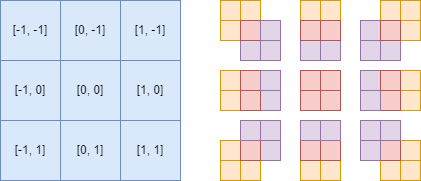
\includegraphics[width=0.6\textwidth]{img/cc.png}
    \caption{Visual representation of the cross-correlation. Yellow and purple matrices correspond to the input matrices, and the blue matrix depicts the cross-correlation output. The coordinates on the blue matrix correspond to the shift of the yellow matrix, which is depicted on the right. Only the overlapping parts (in pink) contribute to the computation for each output matrix element.}
    \label{fig:cross-correlation}
\end{figure}

\subsection{Implementation}

The definition-based approach is a straightforward implementation of the cross-correlation formula. It is a simple algorithm that computes the dot product for all $(2w - 1) \cdot (2h -1)$ overlaps of input matrices. The algorithm is highly parallelizable but suffers from a relatively significant workload imbalance (since each overlap comprises a different number of matrix elements) and a low baseline arithmetic intensity if we do not consider any data-sharing techniques. 

\paragraph{Irregular workload} In our work, we addressed this issue by experimenting with different workers. Having multiple levels of parallelism on contemporary GPUs allows us to experiment with different `work groups' to assign them to a single overlap computation. Generally, we can choose from a \emph{warp}, a \emph{block}, or a \emph{grid} of threads on CUDA platform (in the hierarchically ascending order)\footnote{The most recent versions of CUDA introduces one more group of threads hierarchically located between a block and a grid called a \emph{block cluster}.}. They all have different ways to synchronize and share data, with a typically increasing penalty as we ascend the hierarchy. Notably, threads in a warp support data-sharing constructs within the fastest memory on a GPU --- the register file. 

In our work, we analyzed the memory traces produced by fetching the data during the computation of the neighboring overlaps. A usable memory pattern emerges if the overlapping data is read in a typical row-major pattern. A thread $t$ in iteration $i$ requires the same data as a thread $t-1$ at iteration $i-1$. Such a pattern favors the warp-level parallelism with high-throughput shuffle intrinsics, which allow for shuffling data within thread registers. In our work, we utilized the \emph{register buffer} to read ahead the data for immediate sharing.

Such work distribution enabled a moderate baseline for data sharing, increasing the arithmetic intensity of the algorithm. We also experimented with other work groups, such as assigning multiple threads or the whole block to a single overlap computation. This helped when the overall achievable parallelism was low when processing extremely small inputs.

\paragraph{Data sharing} To further increase the arithmetic intensity, we experimented with other data-sharing techniques that the problem allowed, such as sharing the same overlapping elements between neighboring overlaps. In a \emph{one-to-many} use case, where cross-correlation is computed between one left matrix and multiple right matrices, data loaded from the left matrix can be shared among multiple right matrix overlaps. Respectively, in the \emph{n-to-m} use case, the same can be done with the right matrix. 

Notably, all the mentioned sharing techniques are orthogonal to each other and can be freely combined. Naturally, the growing register requirements with each combined technique are bounded by a limit in the size of the register file (typically around 64KB) and the number of registers, which can be assigned to a single thread by a compiler. If the limit is reached, occupancy drops or register spilling occurs. Apart from that, one also has to consider the decreased parallelism that inherently comes with data sharing.

Therefore, to find the perfect balance between data sharing and the level of parallelism, we conducted a thorough benchmarking process and created the optimization matrix for the cross-correlation algorithm. It generally showed, that the high-overhead FFT implementation provides plenty of space for the definition-based approach to shine, even on a moderately sized n-to-m problem instances.


\section{Stochastic simulation of Boolean networks}

In the last section of this chapter, we will discuss the challenges of porting a stochastic simulation of Boolean networks to GPUs. 

another domain of scientific algorithms

the mission is the same -> enable more research by improving the performance

describe the simulation

talk about the challenges  
- iteration step is not suitable for GPUs 










% thesis is organized as follows

% tam pridat paragraf ku kazdemu clanku

% a az na koniec 1

% viac zrovnanie

% preco su tieto alg tazke

% pitfally co sa stanu ked implementujes na gpu

% v inter tiez dokladne povedat preco to mame rozdelene na scientific aglos + noarr



% gPu science
% - ukazat preco je to zaujimave
% - ze to je potrebne pre biologov
% - ze to zlepsuje situaciu pre vyskum
% - ze je to zaujimavy problem - takze asi spomenut ake boli doterajsie limitacie
% - ukazat ze to je fakt tazky - popisat, co si to vyzadovalo, ake to malo problemy, ma to vela moznosti kde to paralelizovat, vsetky popisat 
% - ale na vysokej urovni - zhrnut a vysvetlit ze to je tazke
% - na zaver poplacat na zadech - zrychlili sme to 1000x

% - future work skor nie 
% - 

% ku intur hodit referencie idealne surveye
